\documentclass[10pt,a4paper]{article}
\usepackage[utf8]{inputenc}
\usepackage[italian]{babel}
\usepackage{amsmath}
\usepackage{amsfonts}
\usepackage{amssymb}
\usepackage{graphicx}
\usepackage[left=2cm,right=2cm,top=2cm,bottom=2cm]{geometry}
\newcommand{\rem}[1]{[\emph{#1}]}

\author{Gruppo AC \\ Federico Belliardo, Giulia Franchi, Francesco Mazzoncini}
\title{Esercitazione N.7: Usi non lineari dell’ OpAmp}
\begin{document}

\maketitle
Questa esperienza ha come obbiettivo quello di studiare il funzionamento di un amplificatore operazionale modello TL081 in circuiti non lineari.

\section*{A. Discriminatore}

Si è montato il circuito in figura\ref{circuito1}, utilizzando $V_{CC} = 14.96\pm0.08 \, V$ e $V_{EE} = 14.96 \pm 0.08 \, V$ come tensioni di alimentazione.

\begin{figure}[h]
\centering
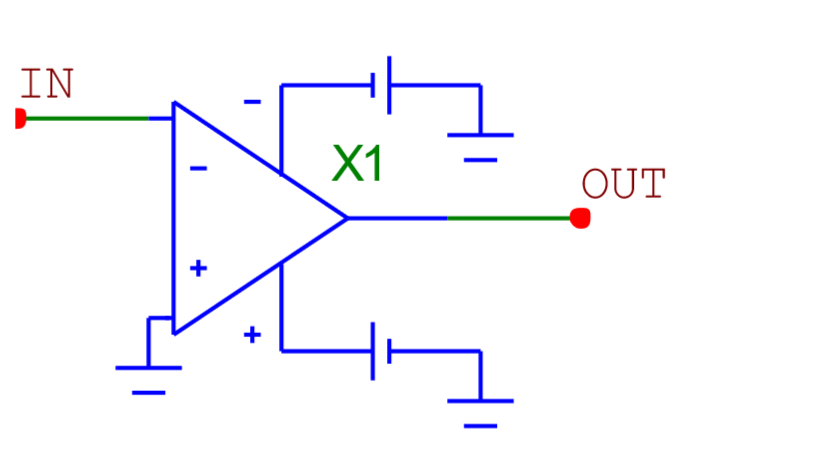
\includegraphics[scale=0.5]{Discriminatore.png}
\caption{Discriminatore realizzato con un OpAmp modello TL081.}
\label{circuito1}
\end{figure}

Si è poi proseguito con lo studio della risposta del circuito ad un segnale sinusoidale. Il circuito ideale dovrebbe funzionare come un comparatore. Se così fosse, il segnale in ingresso verrebbe invertito e amplificato e l'amplificatore, a causa del grande guadagno dell'operazionale, andrebbe in saturazione restituendo un segnale uguale alla tensione di alimentazione ( $V_{EE}$ per un segnale positivo e $V_{CC}$ per uno negativo).\\
Per basse frequenze il comportamento è quello ideale del discriminatore (l'uscita è un'onda quadra), come si vede in fig.\ref{funzionaBene}.

\rem{prendere questa immagine!}
\rem{aggiungere immagine discriminatore che funziona.}

Purtroppo il circuito da noi analizzato non è un amplificatore ideale e come tale presenta dei limiti al suo funzionamento.\\
Come primo limite vediamo l'influenza della tensione di offset $V_{OS}$, che dalla fig.\ref{Vos} è stimata essere $V_{OS} = 25.6 \pm 0.8 \, mV$.\\

\begin{figure}[h]
\centering
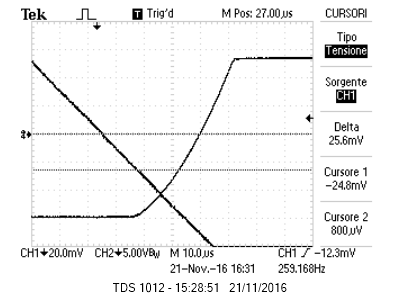
\includegraphics[scale=1.0]{immagini/Vos.png}
\caption{Misura della tensione di offset $V_{os}$}
\label{Vos}
\end{figure}

Inoltre all'aumentare della frequenza si notano gli effetti dello \emph{slew rate} finito dell'OpAmp. La pendenza delle rette che costituiscono la transizione tra uscita alta e bassa satura e il segnale diventa sempre più simile a un onda trapezoidale, per diventare poi un'onda triangolare, vedi fig.\ref{slewRate}.

\begin{figure}[h]
\centering
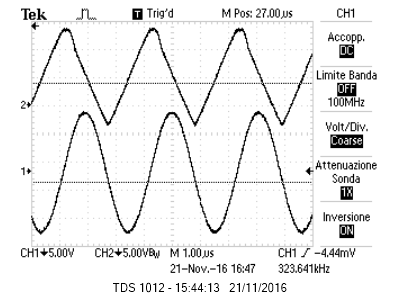
\includegraphics[scale=1.0]{immagini/slewRate.png}
\caption{Effetto dello \emph{slew rate} sull'uscita del disciminatore.}
\label{slewRate}
\end{figure}

Abbiamo valutato lo \emph{slew rate} con due misure di tensione e di tempo: $dV = 4.00 \pm 0.04 \, V$ e $dt = 336 \pm 4 \, ns$, da questa si ricava la misura \emph{slew rate} = $11.9 \pm 0.4 \, \frac{V}{\mu s}$, questo valore è simile a quello trovato nell'esperienza precedente \emph{slew rate} = $11.4 \pm 0.6 \, \frac{V}{\mu s}$.

Ad alta frequenza e a basso segnale si osserva clipping inferiore o superiore del segnale, questo dipende dal segno dell'offset che il generatore di funzioni fornisce, infatti nell'opAmp un segnale a frequenza nulla viene integrato e l'uscita si satura alla tensione di alimentazione che ha segnale opposto (\rem{giusto?}) all'offset, come si vede in fig. \ref{clipping}.\\

\begin{figure}[h]
\centering
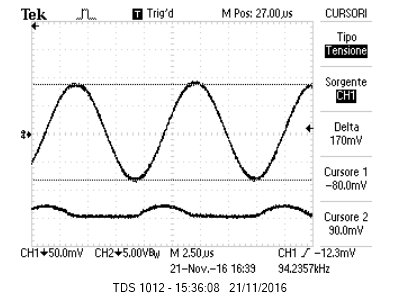
\includegraphics[scale=1.0]{immagini/prodottoBandaGuadagno2.png}
\caption{Clipping del segnale sinusoidale ad alta frequenza.}
\label{clipping}
\end{figure}

Ad alte frequenze il circuito si comporta da integratore (\rem{quale è l'impedenza che mi da la tensione di taglio?}, dunque il segnale in uscita è sinusoidale e, si può scegliere l'offset del generatore in modo che l'uscita non saturi mai e il circuito si comporti perfettamente come un integratore, come si vede nelle figure \ref{senoAlto} e \ref{senoBasso}. L'ampiezza del segnale aumenta al diminuire della frequenza come ci si aspetta per un circuito integratore. 

\begin{figure}[h]
\centering
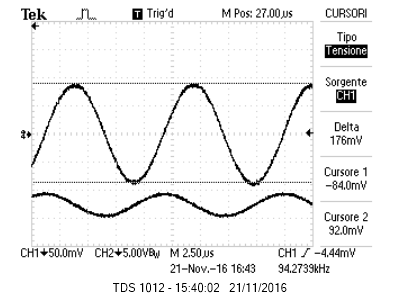
\includegraphics[scale=1.0]{immagini/sinusoidaleinBasso.png}
\caption{Segnale sinusoidale intgrarato con offset (in uscita) in basso.}
\label{senoBasso}
\end{figure}


\begin{figure}[h]
\centering
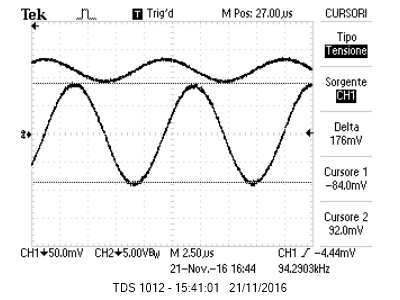
\includegraphics[scale=1.0]{immagini/sinusoidaleinAlto.png}
\caption{Segnale sinusoidale intgrarato con offset (in uscita) in alto.}
\label{senoBasso}
\end{figure}

La finitezza del fattore GBW, intruduce una frequenza di taglio enl sistema e una massima amplificazione alle basse frequenze (che è comunque limitata dalle tensioni di alimentazione). Il seganle in uscita è comunque limitato dalla tensione di alimentazione quindi non si può valutare l'ampificazione massima e pertanto risulta difficile dare un stima del prodotto $GBW = A_{max} * f_{taglio}$.

\section*{B. Amplificatore di carica}

Si è montato il circuito in fig.\ref{circuito2} utilizzando i componenti $C_T = 1.01\pm0.04 \, nF$, $C_F = 1.02 \pm 0.04 \, nF$, $C_1 = 21.9 \pm 0.9 \, nF$, $R_1 = 98.3 \pm 0.8 \, k \Omega$, $R_2 = 99.9 \pm 0.8 \, k\Omega$, $R_3 = 97.8 \pm 0.8 \, k \Omega$ e le tensioni $V_{CC} = 14.96\pm0.08 \, V$ e $V_{EE} = 14.96 \pm 0.08 \, V$. Si è poi regolato il potenziometro $R_3$ in modo che la tensione di soglia del discriminatore fosse ($\sim 200mV$) $V_{R3} = 200 \pm 4 \, mV$ e si è fornita dal generatore di funzioni un'onda quadra.\\

\begin{figure}[h]
\centering
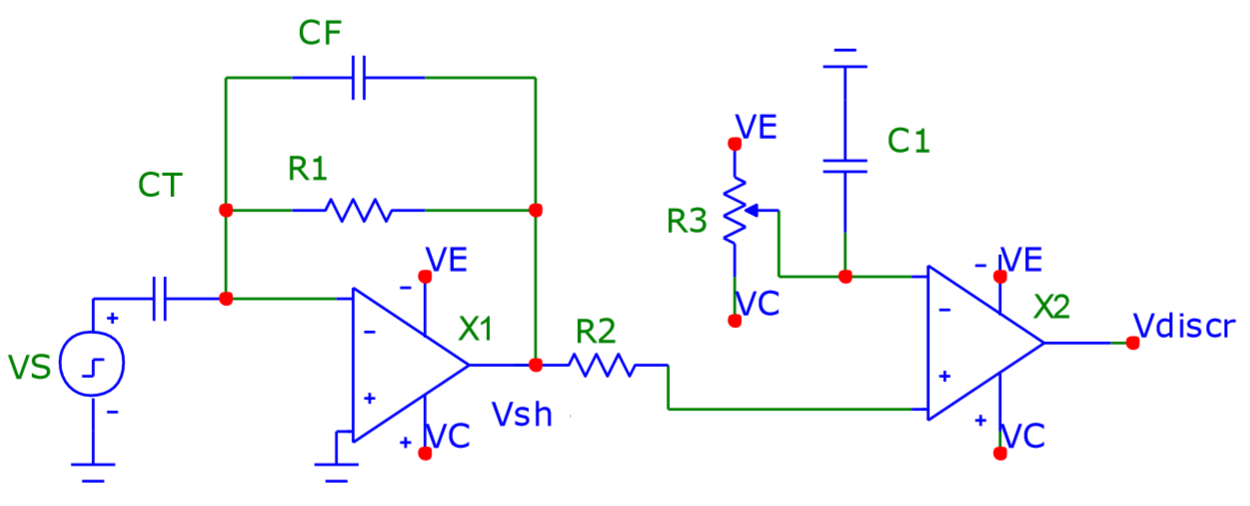
\includegraphics[scale=0.5]{amplificatoreCarica.png}
\caption{Amplificatore di carica realizzato con un OpAmp modello TL081.\label{circuito2}}
\end{figure}

\subsection*{1. Descrizione del circuito e prime misure}
Il circuito montato è costituito da tre parti distinte: un circuito di iniezione di carica ($V_S$+$C_T$), un circuito formatore che converte la carica in un segnale di forma fissata (X1) e un discriminatore che confronta il circuito con una soglia prefissata (X2).

La prima parte è costituita dal generatore di forme d'onda $V_S$ e dal condensatore $C_T$, dove viene fornita una carica pari a $Q_{IN}=V_S C_T$. Il formatore invece è rappresentato dal parallelodi $C_F$ e $R_1$, all'uscita di tale circuito si ha un segnale:\\
\begin{center}
$V_{SH}=\frac{Q_{IN}}{C_F} e^{-\frac{t}{\tau}} = V_S \frac{C_T}{C_F} e^{t/R_1 C_F}$\\
\end{center}

Il resto del circuito rappresenta il discriminatore, analogo a quello descritto al punto A, ma con una tensione di soglia. I componenti $R_2$ e $C_1$ hanno il compito di disaccoppiare il circuito formatore da quello discriminatore e di ridurre il rumore sulla tensione di soglia ad alte frequenze.\\
A frequenza fissata $f = 100\pm 1 \, Hz$ si è misurata la risposta del circuito ad un segnale di ampiezza picco-picco $V_S = 6.00 \pm 0.04 \, V$.\\
L'ampiezza massima attesa per il segnale $V_{SH}$, secondo la formula sopra citata, è $V_{SH.MAX.ATT} = V_S \frac{C_T}{C_F} =  5.9 \pm 0.3 \, V$, mentre il valore misurato sperimentalmente è $V_{SH.MAX} = 5.72 \pm 0.04 \, V$, come si vede in figura \ref{esponenziale}.\\

\begin{figure}[h]
\centering
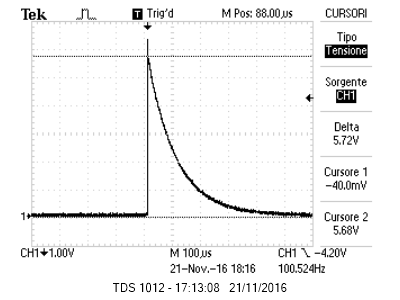
\includegraphics[scale=1.0]{immagini/esponenziale.png}
\caption{Misura del massimo valore dell'esponenziale $V_{SH.MAX.}$}
\label{esponenziale}
\end{figure}

Si sono misurati sull'oscilloscopio il tempo impiegato dal'esponenziale a scendere sotto i  $200 \, mV$ (fig. \ref{tempoEspo}) e il tempo per cui il segnale di uscita è alto (\ref{tempoUscita}), i due valori sono $t_1 = 340 \pm 4 \, \mu s$ e  $t_2 = 336 \pm 4 \mu s$ rispettivamente, i due valori di tempo sono compatibili tra di loro.

\begin{figure}[h]
\centering
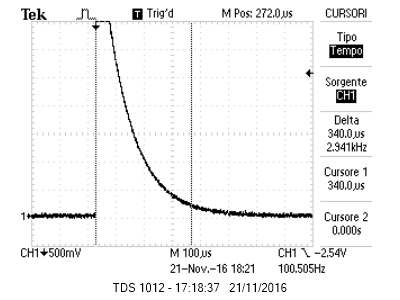
\includegraphics[scale=1.0]{immagini/periodoEsponenziale.png}
\caption{Tempo $t_1$ impiegato dall'ingresso del discriminatore a scendere sotto soglia.}
\label{tempoEspo}
\end{figure}

\begin{figure}[h]
\centering
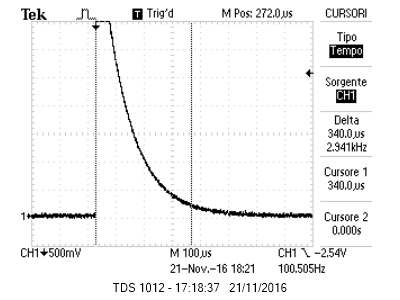
\includegraphics[scale=1.0]{immagini/periodoEsponenziale.png}
\caption{Tempo in cui l'uscita del discriminatore si mantiene positiva.}
\label{tempoUscita}
\end{figure}

\rem{Dire perchè il condensatore si arica a +6 e non a +3!!}


\subsection*{2. Dipendenza del segnale in uscita dall'ampiezza del segnale in ingresso}

Sempre mantenendo una frequenza fissa $f = 100 \pm 1 \, Hz$, si è misurata, al variare dell'ampiezza, la durata nel tempo del segnale in uscita dal discriminatore, i dati sono riportati nella tabella seguente.

\begin{table}[!ht]
\centering
\begin{tabular}{|c|c|c|c|}
\hline 
• & $V_{IN} (V)$ & $\Delta t _ {atteso} (\mu s)$ & $\Delta t _ {misurato} (\mu s)$ \\ 
\hline 
1 & $6.00 \pm 0.06$ & $340 \pm 10$ & $336 \pm 4$ \\ 
\hline 
2 & $4.00 \pm 0.04$ & $300 \pm 10$ & $293 \pm 4$ \\ 
\hline 
3 & $2.00 \pm 0.01$ & $230 \pm 8$ & $220 \pm 4$ \\ 
\hline 
\end{tabular} 
\end{table}

Dalla $V_-=V_S \frac{C_T}{C_F} e^{- \Delta t/R_1 C_F}$, si ottiene $\Delta t = -R_1 C_F log\left( \frac{V_- C_F}{V_S C_T}\right)$, i valori di tempo attesi sono riportati in tabella, insieme a quelli misurati, si può riscontrare che vi è accoro entro l'errore.

Per una tensione in ingresso (massimo valore di $330 \, mV$ si vede che il segnale in uscita dall'amplificatore di carica perde la forma d onda quadra e incomincia a diventare sinusoidale (fig. \ref{inizamorire}), per una tensione in ingresso che scende sotto il valore di soglia di $200 \, mV$ il trigger non si attiva, come si vede in figura \ref{morto}.

\begin{figure}[h]
\centering
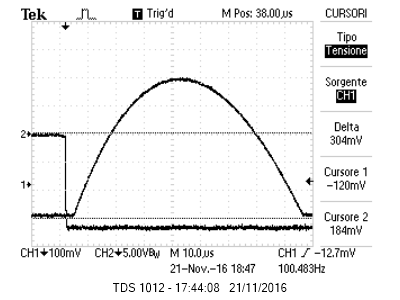
\includegraphics[scale=1.0]{immagini/iniziaamorire.png}
\caption{Tensione in ingresso al trigger del valore di $300 \, mV$.}
\label{inizamorire}
\end{figure}

\begin{figure}[h]
\centering
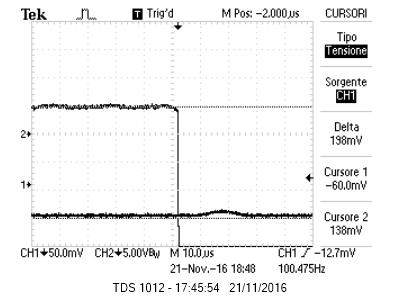
\includegraphics[scale=1.0]{immagini/morto.png}
\caption{Tensione in ingresso al trigger del valore di $300 \, mV$.}
\label{inizamorire}
\end{figure}

\rem{Analisi dati}

\section*{C. Trigger di Schmitt}
\subsection{1. Montaggio, descrizione del circuito e valutazione tensioni di soglia}
Si è montato il circuito in figura\ref{circuito3} con $R_1 = 9.92\pm0.08 \, k\Omega$ e $R_2 = 2.14 \pm 0.03 \, k\Omega$, alimentando l'operazionale con $V_{CC} = 14.96\pm0.08 \, V$ e $V_{EE} = 14.96 \pm 0.08 \, V$.\\

Al circuito è stata inviata una tensione sinusoidale a frequenza di circa $f \sim 710 \pm 7 \, Hz$, e si sono misurate le tensioni in uscita nei due stati possibili del circuito: $V_{OH} = 14.5\pm 0.2 \, V$ e $V_{OL} = 14\pm0.2 \, V$, dalle quali si sono ricavati i valori attesi per le tensioni di soglia $V_{1,ATT,TH}= -V_{OH}/(1+R_1/R_2)= -2.57 \pm 0.05 \, V$ e $V_{2,ATT,TH}= V_{OL}/(1+R_1/R_2) = 2.48 \pm 0.05 V$. 

('Threshold inferiore = ', -2.5729684908789388+/-0.05247901886859559)
('Threshold superiore = ', 2.48424543946932+/-0.05150486638323011)


\begin{figure}[h]
\centering
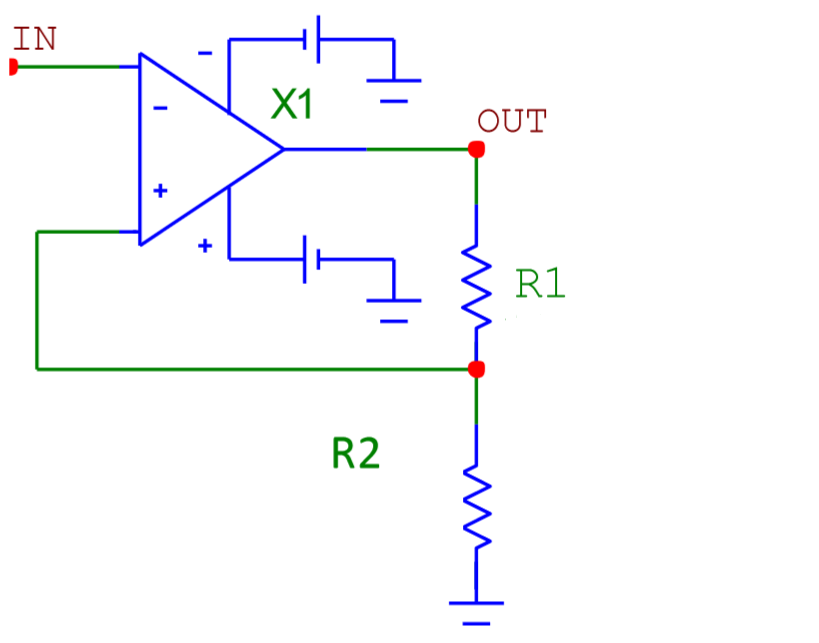
\includegraphics[scale=0.5]{triggerSchmitt.png}
\caption{ Trigger di Schmitt realizzato con un OpAmp modello TL081.\label{circuito3}}
\end{figure}

Questo circuito è un trigger di Schmitt, ovvero un circuito discriminatore con isteresi e reazione positiva.\\

\rem{aggiungere breve funzionamento}

Dalle immagini fig.\ref{sogliameno} e fig.\ref{sogliapiu}, misurando a quale tensione di ingresso di ha la comutazione dell'uscita si sono trovati a due valori per le soglie: $V_{th, -} =-2.60 \pm 0.04 \, V $ e $V_{th, +} = +2.48 \pm 0.04 \, V$.

\begin{figure}[h]
\centering
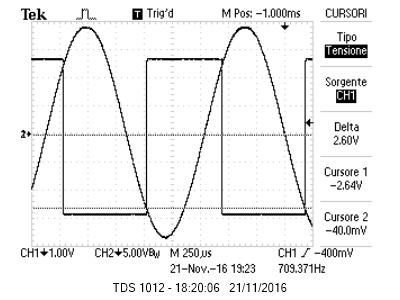
\includegraphics[scale=0.5]{immagini/FotoRicordoVth1.png}
\caption{Misura della soglia inferiore del trigger.}
\label{sogliameno}
\end{figure}

\begin{figure}[h]
\centering
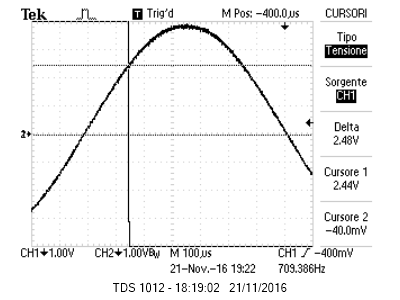
\includegraphics[scale=0.5]{immagini/FotoRicordoVth2.png}
\caption{Misura della soglia superiore del trigger.}
\label{sogliapiu}
\end{figure}

I valori delle tensioni di \emph{threshold} misurati sono in accordo con quelli stimati teoricamente.

\subsection*{2. Dipendenza dall'ampiezza e dalla frequenza e limiti del circuito}

Diminuendo l'ampiezza del segnale in ingresso questo non attraversa mai le soglie del trigger, come si vede nella figura \ref{sottoSoglia}.

\begin{figure}[h]
\centering
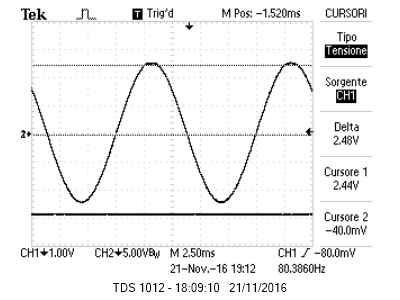
\includegraphics[scale=0.5]{immagini/sottoSogliaInferiore.png}
\caption{Segnale in ingresso che non attraversa le soglie del trigger.}
\label{sogliapiu}
\end{figure}

Il trigger funzionava se la frequenza era invece aumentata.

\section*{D. Multivibratore astabile}
\subsection*{1. Analisi e montaggio del circuito}

Un circuito multivibratore astabile come quello in figura\ref{circuito4} può essere realizzato partendo dal trigger di Schmitt e inserendo componenti nuovi: una resistenza $R$, un condensatore $C$ e due diodi Zener T11N753A.

\begin{figure}[h]
\centering
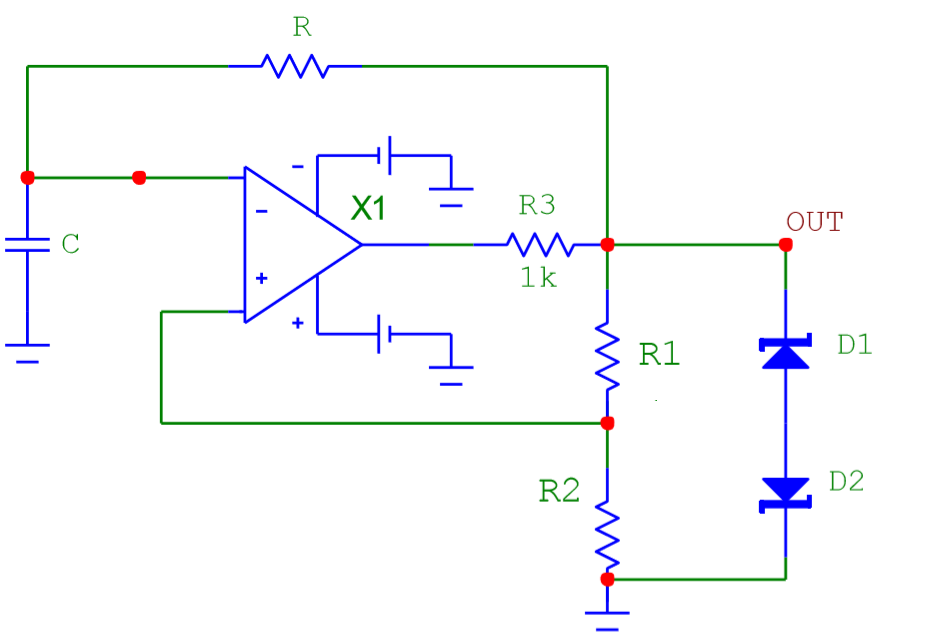
\includegraphics[scale=0.5]{multivibratoreAstabile.png}
\caption{Multivibratore asyabile realizzato con un OpAmp modello TL081.\label{circuito4}}
\end{figure}

\subsection*{2. Breve spiegazione circuito oscillatore}

\begin{figure}[htb!]
\centering
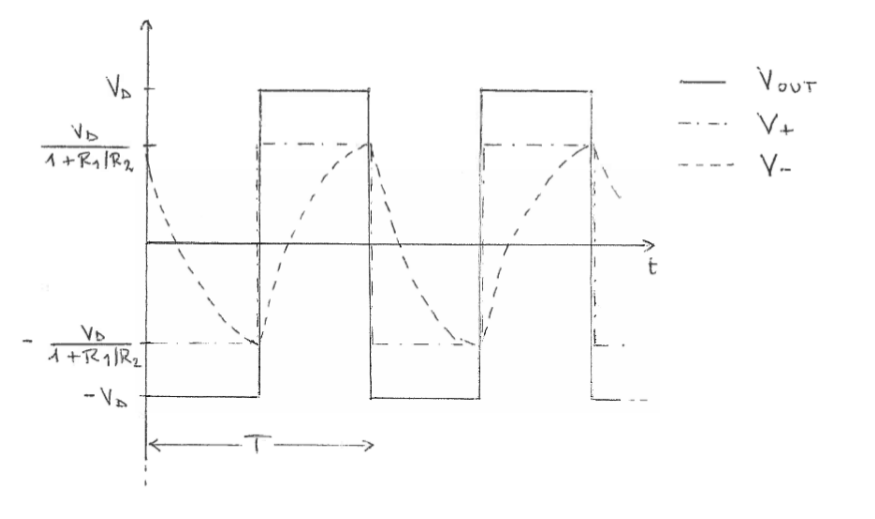
\includegraphics[scale=.5]{funzionamentoOscillatore.png}
\caption{Segnali del multivibratore.}
\label{Vpiu}
\end{figure}

Il condensatore inizialmente carico si scarica sulla resistenza $R$ (infatti il tempo caratteristico dell'oscillazione è determinato da $\tau = RC$), finchè non raggiunge la tensione di \emph{threshold} inferiore del trigger (data da $V_{+}$), allora la tensione in uscita commuta a $+V_{D}$ e anche il \emph{threshold} cambia (trigger di \emph{Schmitt}), il condensatore si carica per raggiungere la tensione $V_D = V_{OUT}$, ma quando raggiunge la tensione di \emph{threshold} superiore l'uscita commuta nuovamente e il condensatore ricomincia a scaricarsi.

Si è determinato il periodo di oscillazione in funzione degli elementi resistivi: 
\begin{center}
$T=2\tau\, log\left( 1\,+\,2\frac{R_2}{R_1}\right) = 1.94 \pm 0.08 \, ms$ 
\end{center}
Dunque per ottenere un periodo dell'onda quadra di $\sim 2 \, ms$ si deve scegliere $\tau = RC\simeq 0.9\,ms$.
A questo punto abbiamo potuto montare il circuito con $R = 3.87 \pm 0.04 \, k\Omega$, e un condensatore $C = 229 \pm 9 \, nF$, $R_1\,= 9.78\pm0.08 \, k\Omega $, $R_2 = 9.80\pm0.08\, k\Omega $ e $R_3 = 0.961\pm0.008 \, k\Omega $, con un' alimentazione per l'OpAmp di $V_{CC} = 14.8 \pm 0.3 \, V$ e $V_{EE} = -14.9 \pm 0.3 \, V$.


\subsection*{3. Verifica funzionamento del circuito}

I diodi Zener servono per limitare la tensione $V_{OUT}$, che satura tra i due valori estremi $\pm V_{D}$, dove $V_{D} = V_{Z} + V_{ \gamma}$. Per il diodo Zener $V_Z \sim 6.2 \, V$ \footnote{Il costuttore non fornisce incertezza.} e $V_{\gamma} \sim 0.7\, V$, dunque $V_D \sim 6.9 \, V$. La tensione in uscita all'opAmp è vincolata alle tensioni di alimentazione ($\pm 15 \, V$), quindi tra l'uscita Zener vi è una caduta di potenziale quindi bisogna inserire una resistenza $R_3$ per evitare che i diodi si brucino a causa del passaggio di corrente elevato.  

Sappiamo che le tensioni di \emph{threshold} superiore e inferiore per il trigger di \emph{Schmitt} sono: $V_{TH} = \pm \frac{V_{D}}{1+\frac{R1}{R2}} = \pm 3.45 \pm 0.05 \, V$, duqnue la tensione picco-picco attesa per il segnale $V_{+, pp} = 6.9 \pm 0.1 \, V$, per il segnale $V_{-}$ ci aspettiamo cicli di carica e scarica del condensatore (quindi funzioni esponenziali) tra le tensioni di \emph{threshold}, quindi $V_{-, pp} = 6.9 \pm 0.1 \, V$. Essendo $V_{OUT}$ variabile tra $+V_{D}$ e $-V_{D}$, ci aspettiamo $V_{OUT, pp} \sim 13.8 \, V$.

Nelle figure \ref{Vpiu}, \ref{Vout}, \ref{Vmeno} si vedono i segnali $V_{+}$, $V_{OUT}$ e $V_{-}$.

\begin{figure}[htb!]
\centering
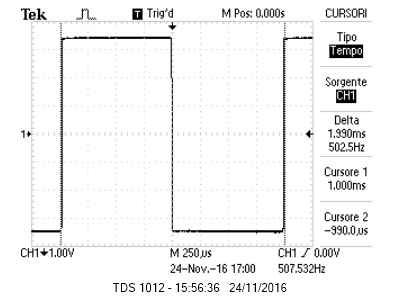
\includegraphics[scale=1.0]{immagini/multivibratoreVPIU.png}
\caption{Segnale $V_{+}$ dell'opAmp.}
\label{Vpiu}
\end{figure}

Il segnale $V_{+}$ è un'onda quadra di ampiezza picco-picco pari a $V_{+, pp} = 6.84 \pm 0.04\, V$, in buon accordo con il valore atteso. Il periodo misurato è $T = 1.99 \pm 0.01 \, ms$, anch'esso in accordo con il valore calcolato teoricamente.


\begin{figure}[htb!]
\centering
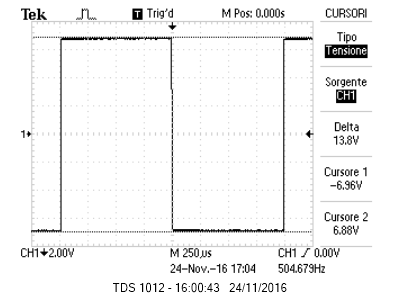
\includegraphics[scale=1.0]{immagini/multivibratoreVOUT.png}
\caption{Segnale $V_{out}$ dell'opAmp.}
\label{Vout}
\end{figure}

Si misura dalla fig.\ref{Vout}: $V_{OUT, pp} = 13.8 \pm 0.1\, V$, in ottimo accordo con quanto atteso.

\begin{figure}[htb!]
\centering
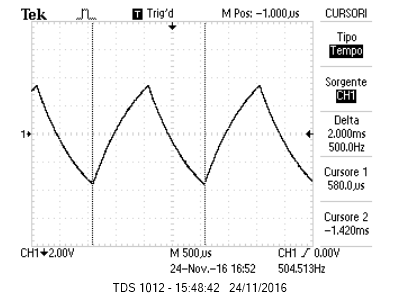
\includegraphics[scale=1.0]{immagini/multivibratoreVMENO.png}
\caption{Segnale $V_{-}$ dell'opAmp.}
\label{Vmeno}
\end{figure}

I tempi di carica e scarica del condensatore sono identici e pari a $t_{salita} = t_{discesa} = 1.00 \pm 0.02\, ms$, e il valore della tensione è: $V_{-, pp} = 6.96 \pm 0.04 \, V$, anche questi valori sono in accordo con quelli attesi.


\subsection*{4. Dipendenza dalla tensione di alimentazione}
Variando la tensione di alimentazione \footnote{Restando nell'intervallo di tensioni di alimentazione indicati dal \emph{datasheet}, cioè non minori di $11\,V$ in valore assoluto.} non osserviamo significative variazioni del periodo dell'oscillatore perchè esso dipende solo dai valori delle resistenze e dei condensatori e non dalle alimentazioni. 


\subsection*{5. Limitazioni alla frequenza del segnale in ingresso}
Il funzionamento ad alta frequenza dell'oscillatore è limitato dallo \emph{slew rate}, in quanto l'opAmp esegue la commutazione tra i valori $\pm V_{D}$ in un tempo finito che deve essere molto minore del periodo di oscillazione del circuito.

\begin{figure}[htb!]
\centering
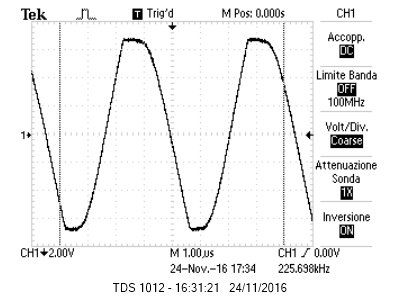
\includegraphics[scale=1.0]{immagini/multivibSlewRate.png}
\caption{Limitazioni dello \emph{slew rate} sul tempo di commutazione.}
\label{slewrate}
\end{figure}

Per osservare abbiamo diminuito il valore di $\tau$ finchè non è diventato confrontabile con il valore del tempo di commutazione come si vede in fig. \ref{slewrate}. Quindi per $C = 0.099 \pm 0.004\, nF$ si è valutata la pendenza del segnale nel tempo di commutazione: $dV = 2.00 \pm 0.04 \, V$ e $dt = 192 \pm 4 \, ns$, da cui \emph{slew rate} = $10.3 \pm 0.3 \, \frac{V}{\mu s}$.\\
Possiamo concludere che l'oscillatore funziona bene per frequenze $f << \frac{1}{t_{commutazione}} \sim \frac{1}{1 \, \mu s} = 1 \, MHz$, infatti il tempo di commutazione come si vede dalla fig. \ref{slewrate} è ci circa $1 \, \mu s$.

\end{document}